\documentclass[12pt,a4paper]{article}
\usepackage[a4paper, margin=0.8in, headheight=14pt]{geometry}
\usepackage{fontspec}
\usepackage{unicode-math}
\setmainfont{TeX Gyre Pagella}
\setmonofont[Scale=0.88]{TeX Gyre Cursor}
\setmathfont{Latin Modern Math}
\usepackage{xcolor}
\usepackage{colortbl}
\usepackage{titlesec}
\usepackage{enumitem}
\usepackage{tabularx}
\usepackage{booktabs}
\usepackage{array}
\usepackage{amsmath}
\usepackage{tikz}
\usetikzlibrary{shapes.geometric, arrows.meta, positioning, calc, fit, decorations.pathreplacing}
\usepackage{tcolorbox}
\tcbuselibrary{skins, breakable}
\usepackage{hyperref}
\usepackage{fancyhdr}
\usepackage{graphicx}
\usepackage{microtype}
\hyphenpenalty=10000
\exhyphenpenalty=10000
\sloppy
\usepackage{caption}
\usepackage{setspace}
\usepackage{multirow}
\usepackage{tocloft}
\newcommand{\Q}[1]{\textbf{#1}\par\noindent\ignorespaces}
\definecolor{myred}{RGB}{196,30,58}
\definecolor{mydark}{RGB}{30,30,50}
\definecolor{mygreen}{RGB}{14,120,80}
\definecolor{myteal}{RGB}{0,130,140}
\definecolor{myamber}{RGB}{180,100,0}
\definecolor{mypurple}{RGB}{100,30,160}
\definecolor{mygray}{RGB}{246,247,249}
\definecolor{mgframe}{RGB}{180,185,200}
\definecolor{watermark}{RGB}{145,150,170}
\definecolor{hdrred}{RGB}{250,232,235}
\definecolor{hdrgreen}{RGB}{220,244,233}
\definecolor{hdrteal}{RGB}{220,242,244}
\definecolor{hdramber}{RGB}{253,242,215}
\definecolor{hdrpurple}{RGB}{238,228,255}
\definecolor{hdrgray}{RGB}{238,240,245}
\definecolor{rowalt}{RGB}{250,251,253}
\titleformat{\section}{\large\bfseries\color{myred}}{\thesection.}{0.5em}{}[\vspace{1pt}{\color{myred}\rule{\linewidth}{0.8pt}}]
\titleformat{\subsection}{\normalsize\bfseries\color{myteal}}{\thesubsection}{0.5em}{}
\titlespacing*{\section}{0pt}{18pt}{7pt}
\titlespacing*{\subsection}{0pt}{11pt}{4pt}
\setlength{\parindent}{0pt}
\setlength{\parskip}{4pt}
\renewcommand{\cfttoctitlefont}{\large\bfseries\color{myred}}
\renewcommand{\cftaftertoctitle}{\par\noindent{\color{myred}\rule{\linewidth}{0.8pt}}}
\setlength{\cftbeforetoctitleskip}{0pt}
\setlength{\cftaftertoctitleskip}{6pt}
\renewcommand{\cftsecfont}{\normalsize\bfseries\color{mydark}}
\renewcommand{\cftsecpagefont}{\normalsize\bfseries\color{mydark}}
\renewcommand{\cftsecleader}{\cftdotfill{\cftdotsep}}
\setlength{\cftbeforesecskip}{7pt}
\renewcommand{\cftsubsecfont}{\small\color{mydark}}
\renewcommand{\cftsubsecpagefont}{\small\color{mydark}}
\setlength{\cftbeforesubsecskip}{3pt}
\setlength{\cftsubsecindent}{1.4em}
\renewcommand{\arraystretch}{1.45}
\setlength{\tabcolsep}{6pt}
\arrayrulecolor{mydark}
\newcolumntype{B}[1]{>{\small\bfseries\raggedright\arraybackslash}m{#1}}
\newcolumntype{Y}{>{\small\raggedright\arraybackslash}X}
\renewcommand{\tabularxcolumn}[1]{m{#1}}
\pagestyle{fancy}
\fancyhf{}
\fancyhead[L]{\small\color{myred}\textbf{PE-EC801B}\;\color{mydark}--- Fiber Optic Communication}
\fancyhead[R]{\small\color{myteal}\textbf{Module 3 Notes}}
\fancyfoot[C]{\small\color{mydark}\thepage}
\fancyfoot[R]{\small\color{watermark}\textit{\copyright\ Biraj}}
\renewcommand{\headrulewidth}{0.5pt}
\renewcommand{\footrulewidth}{0.3pt}
\hypersetup{colorlinks=true, linkcolor=myteal, urlcolor=myteal,
  pdfauthor={Biraj Sarkar}, pdftitle={PE-EC801B --- Module 3 Notes}}
\tcbset{
  tikzbox/.style={colback=mygray, colframe=mgframe, boxrule=0.6pt, arc=4pt,
    left=8pt, right=8pt, top=6pt, bottom=6pt,
    colbacktitle=mgframe, coltitle=mydark, fonttitle=\small\bfseries},
  defbox/.style={colback=hdrgreen, colframe=mygreen, boxrule=0.8pt, arc=4pt,
    left=9pt, right=9pt, top=6pt, bottom=6pt,
    colbacktitle=mygreen, coltitle=white, fonttitle=\small\bfseries},
  formulabox/.style={colback=hdrteal, colframe=myteal, boxrule=0.8pt, arc=4pt,
    left=9pt, right=9pt, top=7pt, bottom=7pt,
    colbacktitle=myteal, coltitle=white, fonttitle=\small\bfseries},
  examplebox/.style={colback=hdramber, colframe=myamber, boxrule=0.8pt, arc=4pt,
    left=9pt, right=9pt, top=6pt, bottom=6pt,
    colbacktitle=myamber, coltitle=white, fonttitle=\small\bfseries},
  masonbox/.style={colback=hdrpurple, colframe=mypurple, boxrule=0.8pt, arc=4pt,
    left=9pt, right=9pt, top=6pt, bottom=6pt,
    colbacktitle=mypurple, coltitle=white, fonttitle=\small\bfseries},
  exambox/.style={colback=hdrpurple, colframe=mypurple, boxrule=1pt, arc=5pt,
    left=10pt, right=10pt, top=8pt, bottom=8pt,
    colbacktitle=mypurple, coltitle=white, fonttitle=\bfseries,
    breakable, title after break={\textbf{Frequently Asked / Viva Questions (contd.)}}}
}
\tcbset{breakable}
\tikzset{
  block/.style={rectangle, draw=myteal, fill=hdrteal,
    text width=2.4cm, align=center, minimum height=0.95cm,
    font=\small, rounded corners=3pt, line width=0.7pt},
  redblock/.style={rectangle, draw=myred, fill=hdrred,
    text width=2.4cm, align=center, minimum height=0.95cm,
    font=\small, rounded corners=3pt, line width=0.7pt},
  netnode/.style={rectangle, draw=myteal, fill=hdrteal,
    text width=1.5cm, align=center, minimum height=0.8cm,
    font=\small, rounded corners=3pt, line width=0.7pt},
  sumjunc/.style={circle, draw=myamber, fill=hdramber,
    minimum size=0.62cm, font=\small, line width=0.8pt},
  snode/.style={circle, draw=mypurple, fill=hdrpurple,
    minimum size=0.55cm, font=\footnotesize, line width=0.7pt},
  arrow/.style={-Stealth, thick, color=mydark},
  redarrow/.style={-Stealth, thick, color=myred},
  line/.style={thick, color=mydark}
}

\begin{document}

\begin{center}
  {\LARGE\bfseries\color{myred} PE-EC801B --- Fiber Optic Communication}\\[5pt]
  {\normalsize\color{mydark} Semester VIII \quad$\bullet$\quad 3L:0T:0P \quad$\bullet$\quad 3 Credits}\\[3pt]
  {\normalsize\color{myteal}\textbf{Module 3 Exam Notes}}\\[3pt]
  {\small\color{mydark} CGEC \;$|$\; B.Tech ECE (2023--27) \;$|$\; \textit{Biraj Sarkar}}
\end{center}
\vspace{2pt}
\noindent{\color{myred}\rule{\linewidth}{1.5pt}}
\vspace{2pt}

\hypersetup{linkcolor=mydark}
\tableofcontents
\hypersetup{linkcolor=myteal}
\newpage

% ===============================================================================
\section{Optical Sources --- LED}
% ===============================================================================

\begin{tcolorbox}[defbox, title={\textbf{Light-Emitting Diode (LED)}}]
An LED is a forward-biased p-n junction semiconductor device that emits light by \textbf{spontaneous emission} when electrons recombine with holes. LEDs for fiber optics operate in the 850\,nm, 1310\,nm, or 1550\,nm windows.
\end{tcolorbox}

\subsection{Surface-Emitting vs Edge-Emitting LED}
\begin{itemize}[leftmargin=*, itemsep=3pt]
  \item \textbf{Surface-Emitting LED (SLED / Burrus LED):} Emits light perpendicular to the junction plane. Large emitting area ($\sim$50\,$\mu$m diameter), Lambertian emission pattern, easy to couple to MMSI/MMGI fibers. Modulation bandwidth $\sim$20--100\,MHz.
  \item \textbf{Edge-Emitting LED (ELED):} Emits light parallel to the junction from the cleaved edge of the active stripe. Narrower emission cone, better coupling to single-mode or small-core multimode fibers. Modulation bandwidth $\sim$100--400\,MHz. Output spectrum FWHM $\sim$30--80\,nm.
\end{itemize}

\begin{tcolorbox}[formulabox, title={\textbf{LED Output and Modulation Bandwidth}}]
\[
P_{opt} \propto I_d \cdot \eta_{ext}, \qquad P(\omega) = \frac{P(0)}{\sqrt{1 + (\omega\tau_r)^2}}
\]
Modulation bandwidth: $f_{3dB} = \frac{\sqrt{3}}{2\pi\tau_r}$, where $\tau_r$ is the minority carrier radiative lifetime ($\sim$2--10\,ns).
\end{tcolorbox}

\textbf{Advantages of LEDs:} Simple construction, lower cost, longer lifetime ($>10^7$ hours), linear L-I characteristic, no threshold, operable without temperature control, immune to catastrophic failure.

\textbf{Disadvantages:} Broad output spectrum (large material dispersion), lower output power, slower modulation compared to laser diodes.

% ===============================================================================
\section{Optical Sources --- Laser Diodes}
% ===============================================================================

\begin{tcolorbox}[defbox, title={\textbf{Laser Diode}}]
A \textbf{laser diode} (LD) is a semiconductor p-n junction in which \textbf{stimulated emission} dominates above a threshold current $I_{th}$. It produces coherent, narrow-spectrum, high-power output suitable for SMF and high-speed links.
\end{tcolorbox}

\subsection{Fabry-Perot (FP) Laser}
Uses two cleaved facets as reflective mirrors forming a Fabry-Perot cavity. Oscillation occurs at wavelengths satisfying the resonance condition $L = m\lambda/(2n)$ ($m$ integer). FP lasers are \textbf{multi-longitudinal-mode}; spectrum is a comb of modes separated by $\Delta\lambda = \lambda^2/(2nL)$.

\subsection{DFB (Distributed Feedback) Laser}
A Bragg grating is integrated into the active layer. Feedback is distributed along the cavity. Only the mode satisfying the Bragg condition $\lambda_B = 2n\Lambda$ (where $\Lambda$ is the grating period) is amplified. DFB lasers are \textbf{single-longitudinal-mode}, essential for WDM systems.

\subsection{Rate Equations and Threshold Current}
\begin{tcolorbox}[formulabox, title={\textbf{Laser Rate Equations and L-I Characteristic}}]
Carrier density $N$ and photon density $S$:
\[
\frac{dN}{dt} = \frac{\eta_i I}{eV} - \frac{N}{\tau_n} - Gg_0(N-N_0)S
\]
\[
\frac{dS}{dt} = Gg_0(N-N_0)S + \frac{\beta N}{\tau_n} - \frac{S}{\tau_p}
\]
Threshold current: $I_{th}$ is where gain = loss (photon density starts growing exponentially).
\[
P_{out} = \eta_d \cdot \frac{hf}{e}(I - I_{th}), \quad I > I_{th}
\]
where $\eta_d$ is differential quantum efficiency, $hf$ is photon energy.
\end{tcolorbox}

\begin{tcolorbox}[tikzbox, title={L-I Curve of a Laser Diode}]
\centering
\begin{tikzpicture}[scale=1.0]
  \draw[-Stealth, thick, color=mydark] (0,0) -- (7.5,0) node[right,font=\small] {Current $I$ (mA)};
  \draw[-Stealth, thick, color=mydark] (0,0) -- (0,5.0) node[above,font=\small] {Output Power $P$ (mW)};
  % Below threshold: near-zero output (LED region)
  \draw[very thick, color=myamber] (0,0.1) -- (3.0, 0.4);
  % Above threshold: linear L-I
  \draw[very thick, color=myred] (3.0, 0.4) -- (6.5, 4.2);
  % Threshold marker
  \draw[dashed, thin, color=mgframe] (3.0, 0) -- (3.0, 0.4);
  \node[font=\small\color{myred}, below] at (3.0, 0) {$I_{th}$};
  % Slope annotation
  \draw[thin, -Stealth, color=myteal] (4.8, 2.2) -- (5.5, 3.1);
  \node[font=\scriptsize\color{myteal}] at (4.3, 2.0) {Slope = $\eta_d \frac{hf}{e}$};
  % Region labels
  \node[font=\scriptsize\color{myamber}] at (1.5, 0.7) {LED region};
  \node[font=\scriptsize\color{myred}] at (5.2, 4.5) {Laser region};
\end{tikzpicture}
\end{tcolorbox}

% ===============================================================================
\section{Photodetectors --- PIN Diode and APD}
% ===============================================================================

\begin{tcolorbox}[defbox, title={\textbf{Photodetector --- Responsivity and Quantum Efficiency}}]
A \textbf{photodetector} converts optical power into electrical current via the photoelectric effect. \textbf{Responsivity} $\mathcal{R}$ (A/W) is the photocurrent per unit optical power. \textbf{Quantum efficiency} $\eta$ is the fraction of incident photons that generate electron-hole pairs.
\end{tcolorbox}

\begin{tcolorbox}[formulabox, title={\textbf{Responsivity Formula}}]
\[
\mathcal{R} = \frac{I_p}{P_{opt}} = \frac{\eta e \lambda}{hc} \quad (\text{A/W})
\]
where $\eta$ = quantum efficiency, $e$ = electron charge ($1.6\times10^{-19}$\,C), $\lambda$ = wavelength (m), $h$ = Planck's constant ($6.626\times10^{-34}$\,J$\cdot$s), $c$ = speed of light. \\
Also: $\mathcal{R} = \eta e / (hf)$ where $f = c/\lambda$ is optical frequency.
\end{tcolorbox}

\subsection{PIN Photodiode}
A \textbf{PIN diode} has a lightly doped intrinsic (I) layer between heavily doped P and N regions. The wide depletion region extends across the I layer under reverse bias, allowing efficient absorption of photons over a large volume.

\begin{itemize}[leftmargin=*, itemsep=2pt]
  \item \textbf{Structure:} P$^+$ / I(intrinsic) / N$^+$, reverse-biased.
  \item \textbf{Bandwidth:} Limited by transit time $\tau_{tr} = d/v_d$ and RC time constant. $f_{3dB} \approx 1/(2\pi\tau_{tr})$. Bandwidths up to tens of GHz are achievable.
  \item \textbf{Responsivity:} Typically $\mathcal{R} \approx 0.6$--$0.9$\,A/W at 1300--1550\,nm (InGaAs PIN).
\end{itemize}

\subsection{Avalanche Photodiode (APD)}
An APD operates under high reverse bias where photogenerated carriers gain sufficient energy to ionize more carriers through \textbf{impact ionization} --- the avalanche effect. This provides internal current gain $M$.

\begin{tcolorbox}[formulabox, title={\textbf{APD Gain, Noise, and SNR}}]
APD multiplication gain: $M = I_{APD}/(I_{primary})$. \\
Excess noise factor: $F(M) \approx k_A M + (1 - k_A)(2 - 1/M)$ (McIntyre approximation), \\
where $k_A$ is the ionization ratio ($k_A = \alpha_h/\alpha_e$). \\
For InGaAs APD: $M$ typically 10--30; $k_A \approx 0.4$--$0.7$.
\end{tcolorbox}

\subsection{Noise in Photodetectors}
\begin{itemize}[leftmargin=*, itemsep=3pt]
  \item \textbf{Shot noise:} Due to the quantum nature of photon detection. $\langle i_s^2 \rangle = 2eI_p B$ (PIN); $\langle i_s^2 \rangle = 2eI_p M^2 F(M) B$ (APD), where $B$ is bandwidth.
  \item \textbf{Thermal noise (Johnson noise):} Due to random thermal agitation of electrons in the load resistor $R_L$. $\langle i_T^2 \rangle = 4k_B T B / R_L$, where $k_B = 1.38\times10^{-23}$\,J/K.
  \item \textbf{SNR:}
\[
\text{SNR}_{PIN} = \frac{(\mathcal{R} P_{opt})^2}{2e\mathcal{R} P_{opt} B + 4k_B T B/R_L}
\]
\[
\text{SNR}_{APD} = \frac{(M\mathcal{R} P_{opt})^2}{2eM^2 F(M)\mathcal{R} P_{opt} B + 4k_B T B/R_L}
\]
\end{itemize}

\subsection{Optical Receivers --- Pre-Amplifier Types}
\begin{itemize}[leftmargin=*, itemsep=3pt]
  \item \textbf{High-impedance (HZ) pre-amplifier:} Large $R_L$ minimizes thermal noise, but limits bandwidth due to RC roll-off. Equalizer needed. Best sensitivity.
  \item \textbf{Transimpedance (TIA) pre-amplifier:} Uses feedback resistor $R_f$ to convert photocurrent to voltage. Flat frequency response up to higher bandwidth with good sensitivity. Preferred in practice.
\end{itemize}

% ===============================================================================
\section{Optical Link Design --- BER, Q-Factor, and Receiver Sensitivity}
% ===============================================================================

\begin{tcolorbox}[defbox, title={\textbf{BER and Q-Factor}}]
\textbf{Bit Error Rate (BER)} is the probability that a received bit is in error. The \textbf{Q-factor} is the signal-to-noise amplitude ratio that directly maps to BER. For a Gaussian noise model: $\text{BER} = \frac{1}{2}\text{erfc}(Q/\sqrt{2})$.
\end{tcolorbox}

\begin{tcolorbox}[formulabox, title={\textbf{Link Design Equations}}]
\renewcommand{\arraystretch}{1.55}
\begin{tabularx}{\linewidth}{B{5.0cm} X}
Q-factor & $Q = \displaystyle\frac{I_1 - I_0}{\sigma_1 + \sigma_0}$ \quad ($I_1, I_0$: mean currents for 1, 0) \\[6pt]
BER vs Q & $\text{BER} \approx \displaystyle\frac{1}{2}\text{erfc}\!\left(\frac{Q}{\sqrt{2}}\right) \approx \frac{\exp(-Q^2/2)}{Q\sqrt{2\pi}}$ \\[6pt]
BER $= 10^{-9}$ requires & $Q \approx 6$ \\[4pt]
Quantum limit & $\text{BER}_{QL} = \frac{1}{2}e^{-\eta N_p}$, minimum $N_p \approx 10$ photons/bit \\[6pt]
Receiver sensitivity & Minimum $P_{min}$ (dBm) for target BER \\[4pt]
\end{tabularx}
\end{tcolorbox}

\subsection{Power Penalties}
Power penalties are additional receiver power margins required due to system imperfections beyond the AWGN model.

\par\noindent
{\renewcommand{\arraystretch}{1.55}
\begin{tabularx}{\linewidth}{|B{3.2cm}|Y|Y|}
\hline
\textbf{Penalty Source} & \textbf{Cause} & \textbf{Typical Range} \\
\hline
Modal noise & Mode partition noise in MMF; speckle pattern changes & 0.5--1\,dB \\
\hline
Extinction ratio & Non-zero optical power for ``0'' bit ($r = P_0/P_1 \neq 0$) & 1--2\,dB (for $r = 0.1$) \\
\hline
Timing jitter & Random deviation in bit timing $\Rightarrow$ ISI & 0.5--2\,dB \\
\hline
Chromatic dispersion & Pulse broadening causes ISI at high bit rate & Depends on $D \cdot B \cdot L$ \\
\hline
Reflection noise & Multiple reflections create interferometric noise & 0.5--1\,dB \\
\hline
\end{tabularx}}

\begin{tcolorbox}[tikzbox, title={Block Diagram --- Complete Fiber Optic Link}]
\centering
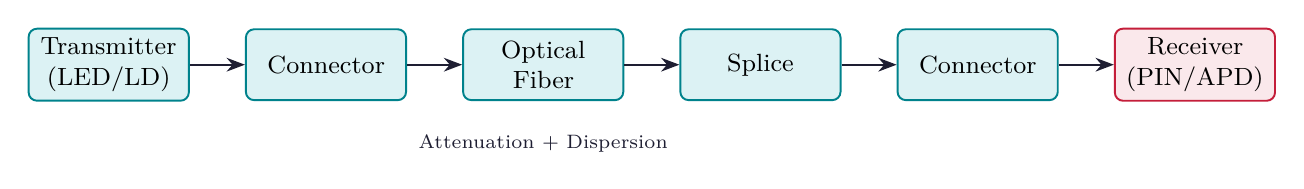
\begin{tikzpicture}[node distance=0.3cm and 0.5cm,
  sblock/.style={rectangle, draw=myteal, fill=hdrteal, text width=1.8cm,
    align=center, minimum height=0.9cm, font=\small, rounded corners=3pt, line width=0.7pt},
  rblock/.style={rectangle, draw=myred, fill=hdrred, text width=1.8cm,
    align=center, minimum height=0.9cm, font=\small, rounded corners=3pt, line width=0.7pt}]
  \node[sblock] (tx) {Transmitter\\(LED/LD)};
  \node[sblock, right=0.7cm of tx] (conn1) {Connector};
  \node[sblock, right=0.7cm of conn1] (fiber) {Optical\\Fiber};
  \node[sblock, right=0.7cm of fiber] (splice) {Splice};
  \node[sblock, right=0.7cm of splice] (conn2) {Connector};
  \node[rblock, right=0.7cm of conn2] (rx) {Receiver\\(PIN/APD)};
  \draw[arrow] (tx) -- (conn1);
  \draw[arrow] (conn1) -- (fiber);
  \draw[arrow] (fiber) -- (splice);
  \draw[arrow] (splice) -- (conn2);
  \draw[arrow] (conn2) -- (rx);
  \node[font=\scriptsize, color=mydark, below=0.3cm of fiber] {Attenuation + Dispersion};
\end{tikzpicture}
\end{tcolorbox}

% ===============================================================================
% QUICK REVISION PAGE
% ===============================================================================
\newpage
\begin{center}
  {\large\bfseries\color{myred} Quick Revision --- Module 3}\\[3pt]
  {\small\color{mydark} Optical Sources, Detectors, and Link Design $|$ PE-EC801B}
\end{center}
\noindent{\color{myred}\rule{\linewidth}{1.2pt}}
\vspace{4pt}

\begin{tcolorbox}[formulabox, title={\textbf{Key Formulas at a Glance}}]
\renewcommand{\arraystretch}{1.35}
\begin{tabularx}{\linewidth}{B{5.0cm} X}
Responsivity & $\mathcal{R} = \eta e \lambda / (hc)$ \quad (A/W) \\[4pt]
Shot noise (PIN) & $\langle i_s^2 \rangle = 2e\mathcal{R}P_{opt}B$ \\[4pt]
Thermal noise & $\langle i_T^2 \rangle = 4k_BTB/R_L$ \\[4pt]
LED modulation BW & $f_{3dB} = \sqrt{3}/(2\pi\tau_r)$ \\[4pt]
Laser output power & $P_{out} = \eta_d(hf/e)(I - I_{th})$ \quad ($I > I_{th}$) \\[4pt]
Q-factor & $Q = (I_1 - I_0)/(\sigma_1 + \sigma_0)$ \\[4pt]
BER (Gaussian) & $\text{BER} = \frac{1}{2}\text{erfc}(Q/\sqrt{2})$ \\[4pt]
BER $= 10^{-9}$ & $Q \approx 6$ \\[4pt]
APD SNR & $\propto M^2 / F(M)$ \quad (optimum $M$ exists) \\[4pt]
\end{tabularx}
\end{tcolorbox}

\begin{tcolorbox}[defbox, title={\textbf{One-Line Definitions}}]
\begin{itemize}[leftmargin=*, itemsep=2pt, topsep=0pt]
  \item \textbf{Spontaneous emission:} Random photon emission by an excited electron without external stimulus (LED).
  \item \textbf{Stimulated emission:} A passing photon triggers an identical photon from an excited state (Laser).
  \item \textbf{Threshold current $I_{th}$:} The bias current above which laser gain exceeds cavity loss.
  \item \textbf{DFB laser:} Distributed Feedback laser; single-mode due to integrated Bragg grating.
  \item \textbf{Responsivity $\mathcal{R}$:} Photocurrent generated per watt of incident optical power (A/W).
  \item \textbf{Quantum efficiency $\eta$:} Fraction of photons that create an electron-hole pair.
  \item \textbf{APD gain $M$:} Internal multiplication of photocurrent by impact ionization.
  \item \textbf{Q-factor:} SNR amplitude ratio; $Q = 6$ gives BER $= 10^{-9}$.
  \item \textbf{Transimpedance amp:} Pre-amplifier with feedback $R_f$ giving flat bandwidth and good sensitivity.
\end{itemize}
\end{tcolorbox}

\begin{tcolorbox}[exambox, title={\textbf{Frequently Asked / Viva Questions}}]
\begin{enumerate}[topsep=0pt, label=\textbf{Q\arabic*.}, itemsep=5pt]
  \item \Q{What is the difference between an LED and a Laser diode?}
    LED uses spontaneous emission; broad spectrum; no threshold; lower power. Laser diode uses stimulated emission above $I_{th}$; narrow coherent spectrum; higher power; higher modulation speed.
  \item \Q{What is the threshold current in a laser diode?}
    It is the minimum bias current at which the gain of the active medium equals the total cavity losses, causing the onset of lasing (stimulated emission dominates).
  \item \Q{Why is a DFB laser preferred for WDM systems?}
    A DFB laser emits a single longitudinal mode (due to the Bragg grating), giving a very narrow linewidth ($<$1\,MHz). This is essential to prevent channel overlap in dense WDM systems.
  \item \Q{Define responsivity and derive the formula $\mathcal{R} = \eta e\lambda/hc$.}
    $\mathcal{R} = I_p/P_{opt}$. Each photon of energy $hf = hc/\lambda$ generates $\eta$ electron-hole pairs, contributing charge $\eta e$. Per second, $P_{opt}/(hf)$ photons arrive, giving $I_p = \eta e P_{opt}/(hf) = \eta e\lambda P_{opt}/(hc)$, so $\mathcal{R} = \eta e\lambda/(hc)$.
  \item \Q{What is the advantage of APD over PIN diode?}
    APD provides internal current gain $M$ through avalanche multiplication, improving receiver sensitivity (lower minimum detectable power). However, it introduces excess noise $F(M)$ and requires higher bias voltage.
  \item \Q{What is shot noise? When is it dominant?}
    Shot noise arises from the discrete quantum nature of photon detection. $\langle i_s^2 \rangle = 2eI_p B$. It dominates over thermal noise at high optical power or when the load resistor is large.
  \item \Q{Define Q-factor and state its relation to BER.}
    $Q = (I_1 - I_0)/(\sigma_1 + \sigma_0)$. For Gaussian noise: $\text{BER} = \frac{1}{2}\text{erfc}(Q/\sqrt{2})$. BER $= 10^{-9}$ requires $Q \approx 6$.
  \item \Q{What is the quantum limit of detection?}
    The absolute minimum BER is set by the Poisson statistics of photon arrival: $\text{BER} = \frac{1}{2}e^{-\eta N_p}$. The quantum limit is $\sim$10 photons/bit for ideal detection.
  \item \Q{What is extinction ratio penalty?}
    When the laser emits non-zero power for a ``0'' bit (extinction ratio $r = P_0/P_1 \neq 0$), the eye opening reduces, requiring extra received power to maintain the same BER. Penalty $= 10\log_{10}\!\left(\frac{1+r}{1-r}\right)$.
  \item \Q{Compare surface-emitting and edge-emitting LEDs.}
    SLED: wide emitting area, Lambertian pattern, easy coupling to MMF, BW $\sim$100\,MHz. ELED: narrow emission cone, better coupling to SMF or small MMF, higher BW $\sim$400\,MHz, higher power.
  \item \Q{What is the difference between high-impedance and transimpedance pre-amplifiers?}
    HZ: large $R_L$ minimizes thermal noise; limited bandwidth needing equalization. TIA: uses feedback $R_f$; flat bandwidth; moderate noise; preferred for practical high-speed receivers.
\end{enumerate}
\end{tcolorbox}

\begin{tcolorbox}[tikzbox, title={LED vs Laser Diode --- Comparison}]
\centering
{\renewcommand{\arraystretch}{1.45}
\begin{tabularx}{\linewidth}{|B{3.2cm}|Y|Y|}
\hline
\textbf{Parameter} & \textbf{LED} & \textbf{Laser Diode} \\
\hline
Emission type & Spontaneous & Stimulated \\
\hline
Coherence & Incoherent & Coherent \\
\hline
Spectral width & 30--80\,nm & $<$1\,nm (DFB) \\
\hline
Threshold & None & $I_{th}$ required \\
\hline
Modulation BW & $\sim$100--400\,MHz & $>$10\,GHz \\
\hline
Output power & Low (mW) & High ($>$10\,mW) \\
\hline
Temperature sensitivity & Low & High \\
\hline
Cost & Low & High \\
\hline
Application & Short-haul, MMF & Long-haul, SMF, WDM \\
\hline
\end{tabularx}}
\end{tcolorbox}

\end{document}
